\documentclass[11pt, wide]{article}
    
    \usepackage[utf8]{inputenc}
    \usepackage[OT4]{polski}
    
    \usepackage{graphicx}
    \usepackage{caption}
    \usepackage{subcaption}
    \usepackage{epstopdf}
    \usepackage{amsmath, amssymb, amsfonts, amsthm, mathtools}
    
    \usepackage{hyperref}
    \usepackage{url}
    \usepackage{bbm}
    \usepackage{comment}
    \usepackage{makecell}
    
    \date{Wrocław, \today}
    \title{\LARGE\textbf{Pracownia z analizy numerycznej}\\Sprawozdanie do zadania \textbf{P2.8}\\
    Prowadzący pracownię: Paweł Woźny}
    \author{Łukasz Klasiński}


    \newtheorem{tw}{Twierdzenie}
    \newtheorem{alg}{Algorytm}

    \begin{document}
    \maketitle
    \thispagestyle{empty}
    \section{Wstęp}
    Problem przybliżania funkcji może być rozwiązany między innymi dzięki
    użyciu interpolacji wielomianowej. Głównym celem niniejszego sprawozdania
    będzie testowanie kilku algorytmów do obliczania wielomianu \textbf{Lagrang'a}, 
    którego postać wygląda następująco:
    \\
    \\
    Wielomian $L_n \in \Pi _n$, spełniający dla danych parami różnych liczb $x_0, x_1, \ldots x_n$ 
    oraz wartości funkcji $f$ w tych punktach, taki że 
    \\\begin{center}
        $L_n(x_k) = f(x_k), (k = 0,1,\ldots,n)$
    \end{center}
    można zapisać w postaci
    \begin{equation}\label{Lagrange}
        L_n(x) = \sum_{i=0}^{n} \lambda_i f(x_i) \prod_{j=0,j\neq i}^{n}(x - x_j)
    \end{equation}
    gdzie
    \begin{equation}
        \lambda_i = \prod_{j=0,j\neg i}^{n}\frac{1}{(t_i - t_j)}
    \end{equation}
    Zbadana zostanie stabilność różnych algorytmów na wybór węzłów oraz jaki generują błąd 
    dla danej ich ilości.
    
    Wszystkie testy numeryczne przeprowadzono przy użyciu języka programowania \textbf{Julia v.0.6.1} w trybie 
    podwójnej (\textbf{Double}) precyzji, czyli 64 bitowej dokładności.
\section{Postać Barycentryczna}
Weźmy równanie (1) i oznaczmy $l_i$ jako $\lambda_i *\prod_{j\neq i}^{n} = \prod_{j\neq i}^{n}\frac{x - x_j}{x_i - x_j} $ z (2)
\\ Zauważmy, że licznik $l_i$ może zostać zapisany jako równość
\begin{equation*}
    l(x) = (x - x_0)(x - x_1)\ldots(x - x_n)
\end{equation*} 
dzielony przez $x - x_i$. Wtedy $\lambda_i = 1/l'(x_i)$, więc $l_i$ można zapisać jako
\begin{center}
    $l_i(x) = l(x)\frac{\lambda_i}{(x - x_i)}$
\end{center}
Zauważmy, że składniki sumy (1) zawierają $l(x)$, który nie zależy od $i$. Dlatego go
wyciągnąć przed sumę, aby otrzymać
\begin{equation}
    L_n(x) = l(x)\sum_{i=0}^{n}\frac{\lambda}{x - x_i}f(x_i)
\end{equation}
Teraz załózmy, że interpolujemy funkcję stałą $ = 1$. Wtedy wstawiając to do (3),
otrzymamy równość                           
\begin{equation*}
    1 = \sum_{i=0}^{n}l_i(x) = l(x)\sum_{i=0}^{n}\frac{\lambda_i}{(x - x_i)}
\end{equation*}
Dzieląc to przez (3), otrzymamy \textsf{barycentryczną formułę} wielomianu (1)
\begin{equation}
    L_n(x) = \frac{\sum_{i=0}^{n}\frac{\lambda}{x - x_i}f(x_i)}{\sum_{i=0}^{n}\frac{\lambda}{x - x_i}}
\end{equation}
dla $\lambda$ takiej samej jak (2). Dalej, przy testowaniu będziemy go nazywać 
\textsf{wielomianem barycentrycznym}.
\\

Zauważmy, że dzięki takiej postaci $\lambda_i$ nie korzysta ze zmiennej $x$.
Dzięki temu dla zadanych węzłów wystarczy raz ją wyliczyć i przy wyznaczaniu wartości
wielomianu używać tej stałej bez ponawiania obliczeń. Ponadto jeśli 
dodamy nowe węzły, to w celu wyliczenia nowej wartości $\lambda_i$, wystarczy
przemnożyć ją przez odpowiedni iloraz $\frac{1}{t_i - t_j}$.
\subsection{Węzły Chebyszewa}
Taka postać wielomianu ma również inną własność. Jeśli zaaplikujemy
do niego węzły Chebyszewa pierwszego rodzaju:
\begin{equation}
x_i = cos\frac{(2i + 1)\pi}{2n + 2}, \hspace*{1cm} (i = 0, \ldots n)
\end{equation}
to wzór na poszczególne wartości $\lambda_i$ z (4) znacząco się upraszcza.
\\
Z własności $\lambda_i = \frac{1}{l'(x)}$, o której była mowa wcześniej, możemy
uzyskać ogólną formułę na $w_i$.
Po zaaplikowaniu do niej węzłów Chebyszewa i usunięciu czynników 
niezależnych od $i$ otrzymamy
\begin{equation}
    \lambda_i = (-1)^j sin\frac{(2j + 1)\pi}{2n + 2}
\end{equation}
Podobnie można postępować w przypadku węzłów Chebyszewa innego rodzaju.
\section{Algorytm Wernera}\label{werner}
Przytoczmy wielomian w postaci Newtona. Wyraża się on wzorem
\begin{equation}
    P_n(x) = \sum_{i=0}^{n}a_i p_i(x)
\end{equation}
gdzie $p_i$ jest wielomianem węzłowym
\begin{equation*}
    p_i(x) = (x - x_0)(x - x_1)\ldots(x - x_{i-1})
\end{equation*}
natomiast współczynniki $a_i$ obliczamy za pomocą ilorazu różnicowego
\begin{equation*}
    a_i = f[x_0,x_1,\ldots,x_i]
\end{equation*}
Główną zaletą tej formy jest mniejsza ilość operacji do wyliczenia wartości
wielomianu w porównaniu do postaci Lagrang'a. Użyjemy tą postać do wyznaczenia algorytmu
wyliczającego $\lambda_i$ w wielomanie barycentrycznym z (4).
\\
Biorąc (1) oraz podstawiając za $f$ funkcję stałą $f(x) = 1$, otrzymamy
\begin{equation}
    1 = \sum_{i = 0}^n\lambda_i\prod_{j=0,j\neq i}^{n}(x - x_i)
\end{equation}
Jeśli rozważymy lewą stronę równania (8) jako wielomian w formie Newtona, to mamy
\begin{equation*}
    P_n(x) = \sum_{i = 0}^n\lambda_i\prod_{j=0,j\neq i}^{n}(x - x_i)
\end{equation*}
Możemy teraz rozwiązać ten wielomian metodą Newtona.
Po przekształceniach tego równania otrzymujemy
\begin{equation*}
    a_k = \sum_{i=0}^{k}\lambda_i\prod_{j=k+1}^{n}(x_i - x_j),\hspace*{1cm} (k = 0, \ldots n)
\end{equation*}
Zatem problem ogranicza się do rozwiązania układu równań:
\begin{equation}
    \left(\begin{array}{c}
        a_0\\
        a_1\\
        a_2\\
        \vdots\\
        a_{n-1}\\
        a_n
    \end{array}\right)
    \left(\begin{array}{ccccc}
        \prod_{j=1}^{n}(x_0 - x_j) & 0 & 0 & \ldots & 0\\
        \prod_{j=2}^{n}(x_0 - x_j) & \prod_{j=2}^{n}(x_1 - x_j) & 0 & \ldots & 0\\
        \prod_{j=3}^{n}(x_0 - x_j) & \prod_{j=3}^{n}(x_1 - x_j) & \prod_{j=3}^{n}(x_2 - x_j) & \ldots & 0\\
        \vdots & \vdots & \vdots & \vdots & \vdots\\
        x_0 - x_n & x_1 - x_n & x_2 - x_n & \ldots & 0\\
        1 & 1 & 1 & \ldots & 1
    \end{array}\right)
    \left(\begin{array}{c}
        \lambda_0\\
        \lambda_1\\
        \lambda_2\\
        \vdots\\
        \lambda_{n-1}\\
        \lambda_n
    \end{array}\right)
\end{equation} 
Może on być rozwiązany za pomocą metody eliminacji Gauss'a, którą zastosujemy w 
innej kolejności niż zwykle:
\begin{enumerate}
    \item Podzielmy pierwsze równanie z (9) przez $x_0 - x_1$, oznaczmy
    \begin{equation*}
        a_0^{(1)} := a_0/(x_0 - x_1)
    \end{equation*}
    \item Odejmijmy pierwsze równianie od drugiego, oznaczmy
    \begin{equation*}
        a_1^{(1)} := a_1 - a_0^{(1)}
    \end{equation*}
    \item Podzielmy pierwsze równianie przez $x_0 - x_2$, oznaczmy
    \begin{equation*}
        a_0^{(2)} := a_0^{(1)}/(x_0 - x_2)
    \end{equation*}
    \item Odejmijmy pierwsze równianie od trzeciego, oznaczmy
    \begin{equation*}
        a_2^{(1)} := a_2 - a_0^{(2)}
    \end{equation*}
    \item Podzielmy drugie równanie przez $x_1 - x_2$, oznaczmy
    \begin{equation*}
        a_1^{(2)} := a_1^{(1)}/(x_1 - x_2)
    \end{equation*}
    \item Odejmijmy drugie równanie od trzeciego, oznaczmy
    \begin{equation*}
        a_2^{(2)} := a_2^{(1)} - a_1^{(2)} 
    \end{equation*}
\end{enumerate}
Kontynując w ten sposób otrzymujemy algorytmu   
\begin{equation}
\begin{aligned}
        &a_k^{(0)} := a_k, \hspace*{1cm} (k = 0,\ldots, n)\\
        &\left.\begin{aligned}
                &a_k^{(i)} := a_k^{(i-1)}/(x_k - x_i)\\
                &a_i^{(k+1)} := a_i^{(k)} - a_k^{(i)}
              \end{aligned}
        \rigth\}
        \qquad k = (0, \ldots, i-1), i = (1, \ldots, n)\\
        &\lambda_i := a_i^{(n)}, \hspace*{1cm} (i = 0, \ldots,n)
\end{aligned}
\end{equation}
Po zastosowaniu go do (8) dostajemy algorytm na wydajne obliczanie 
wartości $\lambda_i$ z (4) 
\begin{equation}
    \begin{aligned}
            &a_0^{(0)} := 0, a_k^{(0)} := 0, \hspace*{1cm} (k = 1,\ldots, n)\\
            &\left.\begin{aligned}
                    &a_k^{(i)} := a_k^{(i-1)}/(x_k - x_i)\\
                    &a_i^{(k+1)} := a_i^{(k)} - a_k^{(i)}
                  \end{aligned}
            \rigth\}
            \qquad k = (0, \ldots, i-1), i = (1, \ldots, n)\\
            &\lambda_i := a_i^{(n)}, \hspace*{1cm} (i = 0, \ldots,n)
    \end{aligned}
\end{equation}
Zatem otrzymaliśmy algorytm Wernera, który pozwala na szybsze obliczenie
wagi barycentrycznej niż w przypadku standardowego wyrażenia. Dzięki temu wykonujemy mniej
operacji i otrzymujemy mniejszy błąd przez utratę cyfr znaczących.
\section{Testy i analiza}
W pierwszym doświadczeniu sprawdzono jak zachowują się poszczególne algorytmy
kiedy zostaną one użyte do interpolacji funkcji wielomianowej. W teori jako, że same
zwracają wielomian, to powinny interpolować ją bezbłędnie. Ale oczywiście jako że działamy na 
liczbach maszynowych, to zwykle otrzymujemy wynik z pewnym błędem. Ten test pokaże, które
algorytmy są na niego bardziej podatne.
\begin{center}
    Interpolujemy funkcję $f(x) = x(x - 3)(x - 2)^2(x - 1)(x + 4)$\\
    na przedziale $[a,b] = [-5,5]$, dla $10 \leq n \leq 500$ węzłów
\end{center}
Poniższa tabelka pokazuje maksymalne błędy bezwzględne w zależności od użytego algorytmu
oraz rodzaju węzłów.
\begin{center}
    TABLICA 1.
\end{center}

\begin{center}
    \begin{tabular}{|c|c|c|c|c|} \hline
        \thead {n} & \thead{Węzły} & \thead{Wielomian \\ Lagrang'a} & \thead{Postać \\ barycentryczna} & \thead{Algorytm \\ Wernera} \\ \hline
        10 & równoodległe & 5.456968e-12 & 1.273293e-11 & 1.818989e-11 \\ \hline
        30 & równoodległe & 2.235829e-07 & 8.321922e-06 & 2.038176e-05 \\ \hline
        50 & równoodległe & 8.546869e-02 & 5.386728e+00 & 3.851245e+00 \\ \hline
        70 & równoodległe & 4.502152e+04 & 2.142437e+06 & 4.819431e+06 \\ \hline
        10 & losowe       & 1.545959e-08 & 1.545959e-08 & 5.140609e-05 \\ \hline
        30 & losowe       & 5.193228e+00 & 3.389305e-07 & 2.355376e+01 \\ \hline
        50 & losowe       & 1.828060e+05 & 7.248581e+03 & 5.629404e+05 \\ \hline
        10 & Chebyszew    & 5.456968e-12 & 5.456968e-12 & 9.094947e-12 \\ \hline
        30 & Chebyszew    & 7.275958e-12 & 5.456968e-12 & 7.275958e-12 \\ \hline
        50 & Chebyszew    & 1.637090e-11 & 5.456968e-12 & 3.829205e-06 \\ \hline        
        70 & Chebyszew    & 2.000888e-11 & 5.456968e-12 & 7.281773e+03 \\ \hline
       500 & Chebyszew    & 5.275069e-11 & 9.094947e-12 & inf            \\ \hline
    \end{tabular}
\end{center}


Jak można zauważyć, w przypadku węzłów równoodległych najlepiej poradził sobie
wielomian Lagrang'a obliczany w standardowy sposób. Jest to prawdopodobnie spowodowane tym,
że jest to "pierwotny" algorytm na znalezienie takiego wielomianu bez żadnych modyfikacji, dzieki czemu
wylicza się najlepiej. Widać również zależność między ilością węzłów a błędem. Od $10$ węzłów
wzwyż wszystkie trzy algorytmy są obarczone coraz większym błędem. Jest on największy
przy krańcach przedziału, co widać na poniższym wykresie:
\begin{center}
    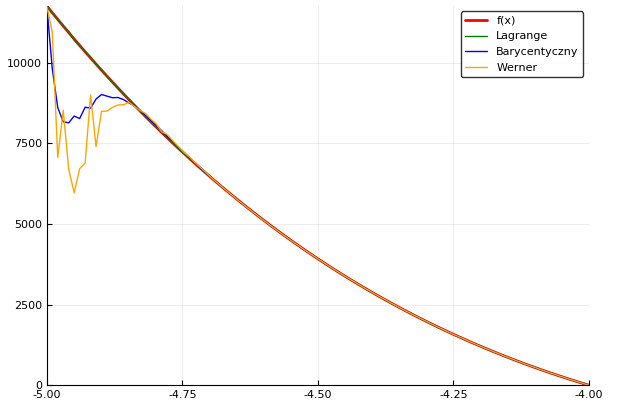
\includegraphics[scale=0.4]{wykres1}\\
    Rysunek 1. $n = 60, [-5,-4]$, węzły równoodległe
\end{center}
Przy węzłach losowych , najmniejszy błąd ma postać barycentryczna. Widać także, że branie
losowych węzłów nie jest najlepszym pomysłem, ponieważ już przy 50 węzłach osiągamy wyniki o wiele gorsze niż w przypadku
równoodległych. Podobnie jak wcześniej tutaj też problemy występują na krańcach przedziału. Z kolei węzły 
Chebyszewa, jak można się było spodziewać powodują w przypadku wielomianu Lagrang'a oraz jego barycentrycznej postaci
minimalne błędy nawet przy bardzo dużej ilości węzłów. Z drugiej strony algorytm Wernera okazuje się znacząco pogarszać
powyżej 30 węzłów.
\begin{center}
    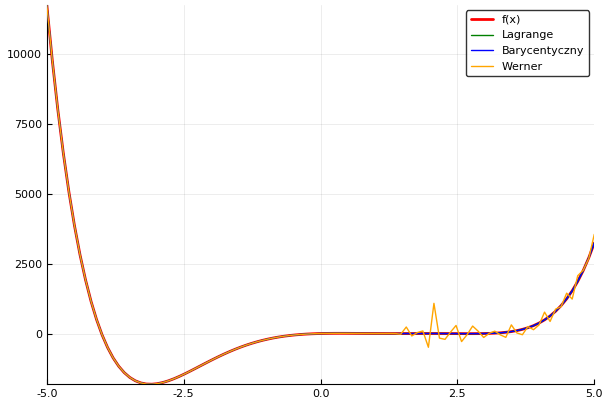
\includegraphics[scale=0.4]{wykres2}\\
    Rysunek 2. $n = 60, [-5,5]$, węzły Chebyszewa
\end{center}
Można zauważyć, że największe błędy algorytmu Wernera są skumulowane po prawej stronie wykresu.
\subsection{funkcja Rungego}
Kolejny test został przeprowadzony na funkcji Rungego, danej wzorem:
\begin{equation*}
    f(x) = \frac{1}{(1 + 25x^2)}
\end{equation*}
$$
[a,b] = [-1,1], 10 \leq n \leq 1000
$$
Jest ona znana z tego, że pomimo zwiększenia ilości węzłów pogarsza się jakość interpolacji wielomianowej, głównie
dla węzłów równoodległych.
Poniżej wyniki:

\begin{center}
    TABLICA 2.
\end{center}
\begin{center}
    \begin{tabular}{|c|c|c|c|c|} \hline
        \thead {n} & \thead{Węzły} & \thead{Wielomian \\ Lagrang'a} & \thead{Postać \\ barycentryczna} & \thead{Algorytm \\ Wernera} \\ \hline
        10 & równoodległe & 1.915643e+00 & 1.915643e+00 & 1.915643e+00 \\ \hline
        30 & równoodległe & 2.277742e+03 & 2.277742e+03 & 2.278585e+03 \\ \hline
        50 & równoodległe & 4.712420e+06 & 4.712025e+06 & 4.712548e+06 \\ \hline
        10 & losowe       & 5.477561e+01 & 5.477561e+01 & 5.477561e+01 \\ \hline
        30 & losowe       & 2.380647e+06 & 2.382197e+06 & 2.905441e+06 \\ \hline
        10 & Chebyszew    & 1.089290e-01 & 1.089290e-01 & 1.089290e-01 \\ \hline
        30 & Chebyszew    & 2.061544e-03 & 2.061544e-03 & 2.061544e-03 \\ \hline
        50 & Chebyszew    & 3.885790e-05 & 3.885790e-05 & 3.885790e-05 \\ \hline        
        70 & Chebyszew    & 7.376980e-07 & 7.376980e-07 & 7.367889e+01 \\ \hline
      1000 & Chebyszew    & 1.788379e+03 & 2.553513e-15 & inf           \\ \hline
    \end{tabular}
\end{center}


Zatem jak można się było spodziewać, węzły równoodległe oraz losowe już od 10 węzłów wykazują
tendencję do pogorszania jakości interpolowania. Natomiast węzły Czebyszewa wręcz przeciwnie. 
Jest to spowodowane ty, że funkcja Rungego powoduje psucie się interpolacji na krańcach przedziału. 
Ponieważ węzły Czebyszewa są gęściej upakowane na końcach przedziału, to negują ten efekt i dla większego $n$ dają rzeczywiście
coraz lepsze przybliżenie. W tym przykładzie wszystkie algorytmy
miały zbliżone błędy oraz zachowanie w stosunku do ilości węzłów nawet przy losowych. Wyjątkiem jest znowu algorytm Wernera,
który dla dużej wartości $n$ podobnie jak wcześniej generuje błędy po prawej stronie wykresu:
\begin{center}
    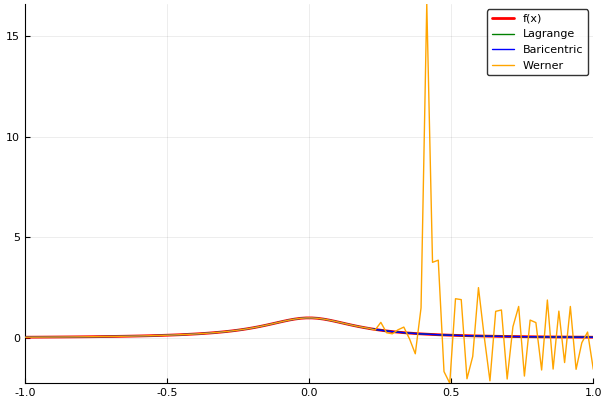
\includegraphics[scale=0.4]{wykres3}\\
    Rysunek 3. $n = 60, [-5,5]$, węzły Chebyszewa
\end{center}
Jak widać w rozdziale (3) algorytm jest wyznaczony
z odpowiednio zbudowanej macierzy. Zatem jest on podatny na błąd spowodowany zbyt dużym 
wyznacznikiem zadania. Dla zbyt dużej ilości
węzłów rośnie on na tyle, ze powoduje takie zabużenia, które widać na wykresie. Warto również
wspomnieć o tym, że przy 1000 węzłów Lagrange zaczął się pogarszać, gdzie postać barycentryczna
była wciąż bardzo dobrym przybliżeniem.
\subsection{funkcja trygonometryczna}
W następnym doświadczeniu wypróbowano interpolacji na funkcji trygonometrycznej.
\begin{equation*}
    f(x) = arctg(x)
\end{equation*}
$$
    [a,b] = [-1,1], 10 \leq n \leq 70
$$
\begin{center}
    TABLICA 3.
\end{center}
\begin{center}
    \begin{tabular}{|c|c|c|c|c|} \hline
        \thead {n} & \thead{Węzły} & \thead{Wielomian \\ Lagrang'a} & \thead{Postać \\ barycentryczna} & \thead{Algorytm \\ Wernera} \\ \hline
        10 & równoodległe & 1.065712e-04 & 1.065712e-04 & 1.065712e-04 \\ \hline
        30 & równoodległe & 2.316384e-09 & 2.474288e-09 & 2.315359e-09 \\ \hline
        70 & równoodległe & 2.593411e+01 & 1.599404e+02 & 7.072912e+00 \\ \hline
        10 & losowe       & 3.956925e-04 & 1.176645e-02 & 1.185675e-04 \\ \hline
        30 & losowe       & 1.484253e-05 & 7.276726e-01 & 4.771568e-02 \\ \hline
        70 & losowe       & 6.075408e+06 & 9.657790e-01 & 1.613932e+00 \\ \hline
        10 & Chebyszew    & 1.477877e-05 & 1.477877e-05 & 1.477877e-05 \\ \hline
        30 & Chebyszew    & 1.214168e-13 & 1.213057e-13 & 1.213057e-13 \\ \hline
        70 & Chebyszew    & 1.776357e-15 & 9.992007e-16 & 2.690387e-01 \\ \hline
       800 & Chebyszew    & 1.398002e+03 & 3.387095e-08 & inf            \\ \hline
    \end{tabular}
\end{center}
Jak widać do interpolowania po funkcji arctg nadają się nawet węzły równoodległe. 
Przy $n = 30$ błąd jest bardzo niewielki i dopiero powyżej zaczyna wzrastać. Jednak w przypadku
węzłów Chebyszewa mamy o wiele lepsze przybliżenie, które utrzymuje się nawet przy dużych ilościach węzłów. Reszta wniosków
jest konsekwentna jak w poprzednich testach.
\subsection{funkcja nieciągła}\label{nieciagla}
Tym razem zastosowano interpolację dla funkcji, która dla danego przedziału nie jest ciągła.
$$
    f(x) = max(0, 1 - 4x)
$$
$$
[a,b] = [-5,5], 10 \leq n \leq 70
$$
Przez to interpolacja będzie miała problemy w przybliżeniu funkcji właśnie w punkcie, gdzie nie 
istnieje pochodna. W tym przypadku $x = \frac{1}{4}$
\begin{center}
    TABLICA 4.
\end{center}
\begin{center}
    \begin{tabular}{|c|c|c|c|c|} \hline
        \thead {n} & \thead{Węzły} & \thead{Wielomian \\ Lagrang'a} & \thead{Postać \\ barycentryczna} & \thead{Algorytm \\ Wernera} \\ \hline
        10 & równoodległe & 3.915349e+00 & 3.915349e+00 & 3.915349e+00 \\ \hline
        30 & równoodległe & 1.591061e+05 & 1.591061e+05 & 1.592003e+05 \\ \hline
        50 & równoodległe & 4.237167e+10 & 4.235769e+10 & 4.036184e+10 \\ \hline
        10 & Chebyszew    & 4.753480e-01 & 4.753480e-01 & 4.753480e-01 \\ \hline
        30 & Chebyszew    & 3.225152e-01 & 3.225152e-01 & 3.225152e-01 \\ \hline
        50 & Chebyszew    & 1.091766e-01 & 1.091766e-01 & 2.927421e+00 \\ \hline
        70 & Chebyszew    & 6.761971e-02 & 6.761971e-02 & 6.681778e+04 \\ \hline
       700 & Chebyszew    & 6.744000e+04 & 7.081382e+00 & inf          \\ \hline    
    \end{tabular}
\end{center}
Przez to, że funkcja nie jest ciągła, to nawet węzły Chebyszewa nie były w stanie osiągnąć 
błędu mniejszego niż $0.07$. Poza tym spowodowało to, że znacznie szybciej niż w
poprzednich doświadczeniach węzły równoległe zaczęły generować szybko rosnący błąd. Poniżej wykres 
przedstawiający interpolację wokół punktu nieciągłości:
\begin{center}
    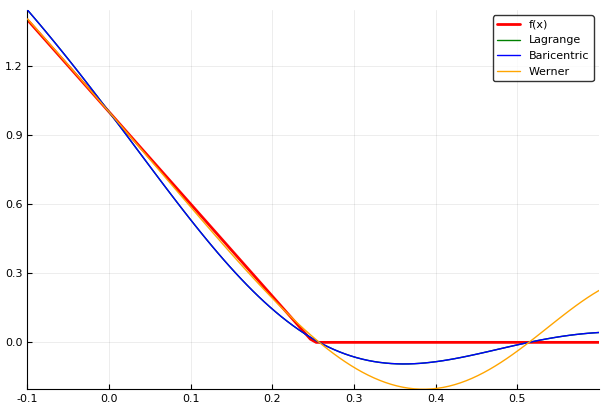
\includegraphics[scale=0.4]{wykres4}\\
    Rysunek 4. $n = 60, [-0.1,0.6]$, węzły Chebyszewa
\end{center}
Widać z niego, że nasz największy błąd był właśnie na prawo od miejsca, gdzie nie istnieje pochodna. 
Pokazuje to zatem, że bardzo ciężko jest interpolować takiego typu funkcji, które nie są ciągłe na danym przedziale.
Poniżej inny ciekawy przykład interpolowania po części ułamkowej $x$ : 
$$
    f(x) = x - floor(x)
$$
który ukazuje problem interpolacji funkcji nieciągłej:
\begin{center}
    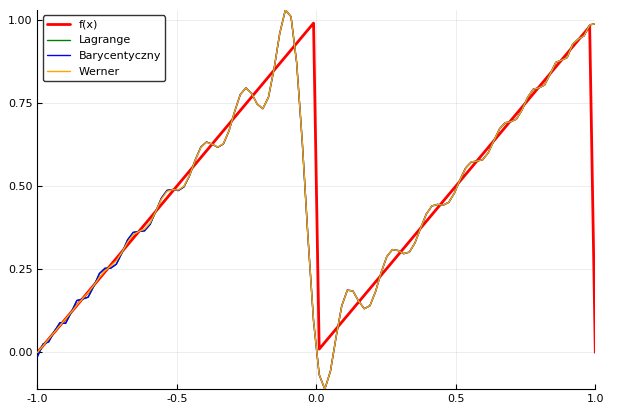
\includegraphics[scale=0.4]{wykres5}\\
    Rysunek 5. $n = 40, [-1,1]$, węzły Chebyszewa
\end{center}
\\

Można zauważyć podobne zachowanie interpolacji jak w przypadku funkcji Rungego - dla węzłów innych
niż Chebyszewa przybliżenie interpolacji wraz ze zwiększeniem węzłów rośnie. I rzeczywiście
takie zachowanie można zauważyć zawsze kiedy funkcja jest nieciągła na danym przedziale.
\section{Podsumowanie}
Po przeprowadzonych eksperymentach, można wywnioskować, że o ile interpolacja
wielomianem Lagrang'a nie jest najepszą - można to zrobić 
z bardzo dobrym przybliżeniem np. funkcjami sklejanymi, to przy odpowiednio dobranych węzłach oraz
ich ilości, można otrzymać całkiem zadowalające rezultaty. Widać to z tablicy (1), (2) oraz (3). Udało się
uzyskać błąd maksymalny rzędu $10^{-15}$. Niestety w przypadku funkcji, które nie są ciągłe, nie jesteśmy już w stanie
uzyskać dobrego przybliżenia, co zostało pokazane w \ref{nieciagla}. Poza tym postać Lagrang'a szybciej od postaci barycentrycznej zaczyna
zwiększać błąd związany ze zbyt dużą liczbą węzłów. Jest to ukazane w każdej tabelce. Natomiast algorytm
Wernera szybko przestawał polepszać przybliżenie funkcji gdy zaaplikowaliśmy do niego więcej niż 50 węzłów. 
Powoduje to, że ma on najlepsze zastosowanie, kiedy nie zależy nam na bardzo precyzyjnych wynikach, ale na szybkości, ponieważ
jak pozaliśmy w rodziale \ref{werner}, wykonuje się on znacznie szybciej w porównaniu do postaci barycentrycznej, a już tym bardziej niż 
postać Lagrang'a. W przypadku kiedy chcemy najlepsze przybliżenie, to należy zastosować algorytm barycentryczny, ponieważ jest szybszy od Lagrang'a a uzyskuje
podobne bądź lepsze rezultaty i jest bardziej stabilny.
\begin{thebibliography}{9}
    \itemsep2pt
    \bibitem{RI} C. Schneider and W. Werner, Some New Aspects of Rational Interpolation 1986
    \bibitem{BLI} J. Berrut and L. N. Trefethen, Baricentric Lagrange Interpolation 2004
    \bibitem{LVN} W. Werner, Polynomial Interpolation: Lagrange versus Newton 1984
\end{thebibliography}    
\end{document}


